\documentclass[a4paper, twoside, 12pt, justified]{article}
\usepackage{lingmacros}
\usepackage{tree-dvips}
\usepackage{graphicx}
\usepackage[T1]{fontenc}
\graphicspath{ {./images/} }
\usepackage{hyperref}
\hypersetup{
	colorlinks=true,
	linkcolor=blue,
}
\usepackage[T1]{fontenc}
\usepackage{mathptmx}
\usepackage[
top=2cm,
bottom=2cm,
inner=3cm,
outer=2cm,
]{geometry}
\usepackage{microtype}

\begin{document}
	
	\begin{figure}[t]
		
\includegraphics[scale=0.8]{AGH}
		\centering
	\end{figure}
	
	\begin{center}
		Wydział Elektrotechniki, Automatyki, Informatyki i Inżynierii Biomedycznej 
		\vspace{10mm} %5mm vertical space
	
		Praca dyplomowa inżynierska \\ 
		\vspace{10mm}
		Optymalizacja trasy z wykorzystaniem algorytmu przybliżonego
	\end{center}
	
	\vfill
	\begin{flushleft}
		Autor: Rafał Siniewicz \newline
		Kieunek studiów: Automatyka i automatyka \newline 
		Opiekun: dr inż. Joanna Kwiecień \newline
	
	\end{flushleft}
	
	\begin{center}Kraków, 2019/2020r.\end{center}
	
	\newpage
	
	\begin{flushleft}
		\begin{large}\textbf{Spis treści}\end{large}
		\textbf{
			\\1. Wstęp }\\
			\hspace{5mm}1.1. Cel pracy\\
			\hspace{5mm}1.2. Zakres pracy\\
			\hspace{5mm}1.3. Wstęp teoretyczny\\
			\textbf{2. Opis projektu}\\
			\hspace{5mm}2.1. Użyte technologie\\
			\hspace{5mm}2.2. Opis aplikacji\\
			\textbf{3. Dokumentacja i działanie aplikacji}\\
			\textbf{4. Testy}\\
			\hspace{5mm}4.1. Sprawdzenie poprawnosci wczytywanych danych\\
			\hspace{5mm}4.2. Dzialanie dla roznych danych i sprawdzenie optymalnosci otrzymanego rozwiazania\\
			\textbf{5. Podsumowanie}\\
		
	\end{flushleft}
	\newpage
	
	%\begin{flushleft}
		
	\begin{flushleft}
		\begin{large}
			\textbf{1. Wstęp }
		\end{large}
	\end{flushleft}
	\vspace{5mm} %5mm vertical space
	
	Transport od zawsze pełnił bardzo ważną rolę w życiu społeczenśtw. W przeciągu wieków zmieniały się środki transpotu, jego metody, a także szybkość przemieszaczania ludzi oraz towarów. Za każdym jednak razem wyzwanie stanowiło jak najoptymalniejsze przeprowadzenie procesu transportu.
	Szczególnie w dzisiejszych czasach zaplanowanie tras w taki sposób, aby zminimalizować czas ich pokonania- co wiąże się z mniejszymi kosztami oraz emisjami spalin- jest bardzo cenne. Również zwyklejsze sytuacje, jak np. zaplanowanie dojazdu do pracy (komunikacją miejską lub samochodem) wymagają od wielu osób skorzystania z odpowiednich narzędzi (świadczy o tym chociażby popularność google maps czy aplikacji jakdojade) przeszukujących wiele możliwych tras i wybierających tą najlepszą. Widać zatem jak dużą rolę odgrywa w życiu niemalże każdego dobranie odpowiedniej trasy dla danej podróży.\\ 
	Problem optymalizacji trasy jest bardzo powszechny i wielokrotnie studiowany, zwłaszcza w badaniach operacyjnych, teorii grafów czy logistyce i dziedzinach pokrewnych. W teorii najczęściej dąży się do uzyskania jak najkrótszej trasy, choć problem można rozwinąć o wiele różnych czynników, które wpływają na przebieg trasy, np. jakość nawierzchni czy określona pojemność pojazdów.
	\vspace{5mm} %5mm vertical space
	
	\begin{flushleft}
		\begin{large}
			\textbf{1.1. Cel pracy}
		\end{large}
	\end{flushleft}
	\vspace{5mm} %5mm vertical space
	
	Praca ma na celu stworzenie aplikacji komputerowej wraz z interfejsem graficznym służącej do obliczania optymalnej trasy na podstawie odpowiednich danych. Optymalna trasa zostanie obliczona przy pomocy odpowiednich algorytmów opisanych w poniższym wstępie teoretycznym. Program będzie również wyświetlał przebiegi tras w formie graficznej wraz z zaznaczeniem poszczególnych punktów na mapie. Całość ma stanowić ujednolicony i łatwy w użyciu system, w którym można ustalać parametry, takie jak, np. ilość pojazdów i ich pojemności, współrzędne geograficzne punktów, a także uzyskać informacje o długości trasy, jej przebiegu i innych statystykach dotyczących rozwiązywanego problemu.  
	\vspace{5mm} %5mm vertical space
	
	\begin{flushleft}
		\begin{large}
			\textbf{1.2. Zakres pracy}
		\end{large}
	\end{flushleft}
	\vspace{5mm} %5mm vertical space
	
	W pracy zagadnienie optymalizacji trasy rozważono dla problemu marszrutyzacji, czyli VRP (Vehicle Routing Problem) oraz CVRP (Capacity Vehicle Routing Problem). Projekt skupia się głównie na dwóch czynnikach decydujących o optymalności: długości trasy oraz zapełnieniu pojazdów ładunkiem. \\
	Przy rozwiązywaniu problemu marszrutyzacji korzystano z algorytmów przybliżonych, a konkretniej algorytmu genetycznego, przede wszystkim ze względu na złożoność problemu, gdyż przy problemach bardziej złożonych dobrze sprawdzają się algorytmy przybliżone.Algorytm genetyczny wybrano również ze względu na jego uniwersalność, możliwość uzyskania stosunkowo dobrych wyników w krótkim czasie oraz prostą koncepcję podejścia do rozwiązania. \\
	
	
	\newpage
	\begin{flushleft}
		\begin{large}
			\textbf{1.3. Wstęp teoretyczny}
		\end{large}
	\end{flushleft}
	\vspace{5mm} %5mm vertical space

	Na podstawie \hyperlink{vrp}{[1]} oraz \hyperlink{cvrp}{[2]}:\\
	VRP (Vehicle Routing Problem)- problem kombinatoryczny bazujący na zbiorach krawędzi i wierzchołków grafu G(V,E). Jest on rozszerzeniem problemu komiwojażera czy problemu chińskiego listonosza. Jest to problem z kategorii NP- trudnych. Notacja: \\
	- V jest zbiorem punktów do odwiedzenia i punktu początkowego,\\
	- E jest zbiorem krawędzi łaczących punkty V,\\
	- d jest wektorem pojemności towarów w punktach,\\
	- k jest liczbą tras,\\
	- C to pojemność pojazdu,\\
	
	Ogólnie dla problemu CVRP rozwiązanie składa się z:\\
	- zbioru \{$R_{1}$,...,$R_{k}$\} z V takiego, że:  $\sum_{j \in R_i} d_j \leq C, \quad 1 \leq i \leq k$ \\
	- permutacji $\theta_i$ z $R_i \cup \{0\}$ określającej kolejność odwiedzonych punktów w trasie $i$\\
	
	Istnieją różne warianty problemu marszrutyzacji, na przykład:\\ 
	- VRP with Time Windows- czyli uwzględnienie okien czasowych odbioru/ wysłania towaru\\
	- Split Delivery VRP- czyli możliwość obsługi jednego klienta przez kilka pojazdów\\
	- Vehicle Routing Problem with Multiple Trips (VRPMT)- czyli możliwość pokonania więcej niż jednej trasy przez jeden pojazd\\
	- Capacitated Vehicle Routing Problem: CVRP- pojazdy mają ograniczoną pojemność\\ 
	- inne

	\vspace{5mm} %5mm vertical space

	Powyższy problem można również rozwinąć o wiele innych czynników, jak np. kolejność odwiedzenia miejsc czy opcjonalnego odwiedzenia niektórych punktów lub funkcja kosztu może rozpatrywać różne parametry, np. czas wykonania zleceń czy ilość przewiezionego ładunku. Widać zatem, że problem marszrutyzacji jest zagadnieniem bardzo rozległym, a przy tym elastycznym, tzn. można go dostosować do wielu różnych problemów.
	
	\vspace{5mm}
	
	Na podstawie \hyperlink{ag}{[3]}:\\
	Termin algorytm genetyczny po raz pierwszy wprowadził John Holland, bazując na koncepcji Darwina- teorii ewolucji. Jest to metaheurystyka (metoda poszukiwania rozwiązań, która nie gwarantuje znalezienia optymalnego rozwiązania) bazująca na zjawisku naturalnej selekcji (teorii ewolucji gatunków), a także dziedziczności. Należy do szerszej grupy- algorytmów ewolucyjnych. Algorytm ten polega na znajdowaniu rozwiązania naśladując zjawiska występujące w środowisku naturalnym, takie jak: mutacje, krzyżowania gatunków, a także selekcja. \newpage
	
	Algorytm genetyczny w krokach:\\
	1. Utworzenie początkowej populacji\\
	2. Przeprowadzanie mutacji i krzyżowania\\
	3. Sprawdzenie funkcji celu dla osobników\\
	4. Wybór najlepszych osobników poprzez selekcję\\
	5. Powtarzanie kroków 2-4 aż do spełnienia warunku stopu\\
	6. Koniec algorytmu i wybór najlepszego osobnika
	
	\vspace{10mm}
	
	
	\begin{figure}[h]
	\includegraphics[scale=0.8]{image}
	\centering
	\\
	{Rysunek1. Schemat algorytmu genetycznego} 
	\end{figure}
	
	
	
	\newpage
	\begin{flushleft}
		\begin{large}
			\textbf{2. Opis projektu}
		\end{large}
	\end{flushleft}
	
	\vspace{5mm} %5mm vertical space
	
	\begin{flushleft}
		\begin{large}
			\textbf{2.1. Użyte technologie}
		\end{large}
	\end{flushleft}
	\vspace{10mm} %5mm vertical space
	
	 Na podstawie \hyperlink{python}{[4]}:\\
	 \textbf{Python}- jest językiem programowania ogólnego przeznaczenia. Jest to język wysokiego poziomu. Może być skutecznie wykorzystywany przy budowie w zasadzie każdego programu. Nie potrzebuje bezpośredniego dostępu do sprzętu komputerowego. Python nie jest optymalny dla programów, które mają duże ograniczenia niezawodności lub są zbudowane i utrzymywane przez wiele osób lub przez długi czas. Ma on jednak kilka zalet w porównaniu z innymi językami programowania, m.in.:\\
	 - jest łatwy w nauce\\ 
	 - posiada bardzo dużą liczbę darmowych i powszechnie dostępnych bibliotek, zapewniających rozszerzoną funkcjonalność\\ \\
	 
	 Na podstawie \hyperlink{osm}{[5]}:\\
	 \textbf{OSM (OpenStreetMap)}- jest to darmowa, edytowalna mapa całego świata, tworzona przez wolontariuszy, wydawana na licencji open-content. Licencja OpenStreetMap pozwala na bezpłatny dostęp do obrazów i podstawowych danych map. Projekt ma na celu promowanie nowych zastosowań tych danych. W pracy OSM zostało wykorzystane do zwizualizowania przebiegów tras i pokazania ich na rzeczywistej mapie. Przykład obrazu uzyskanego dzięki OSM \hyperlink{osm_example}{[6]}: \\
	 
 	\begin{figure}[h]
 	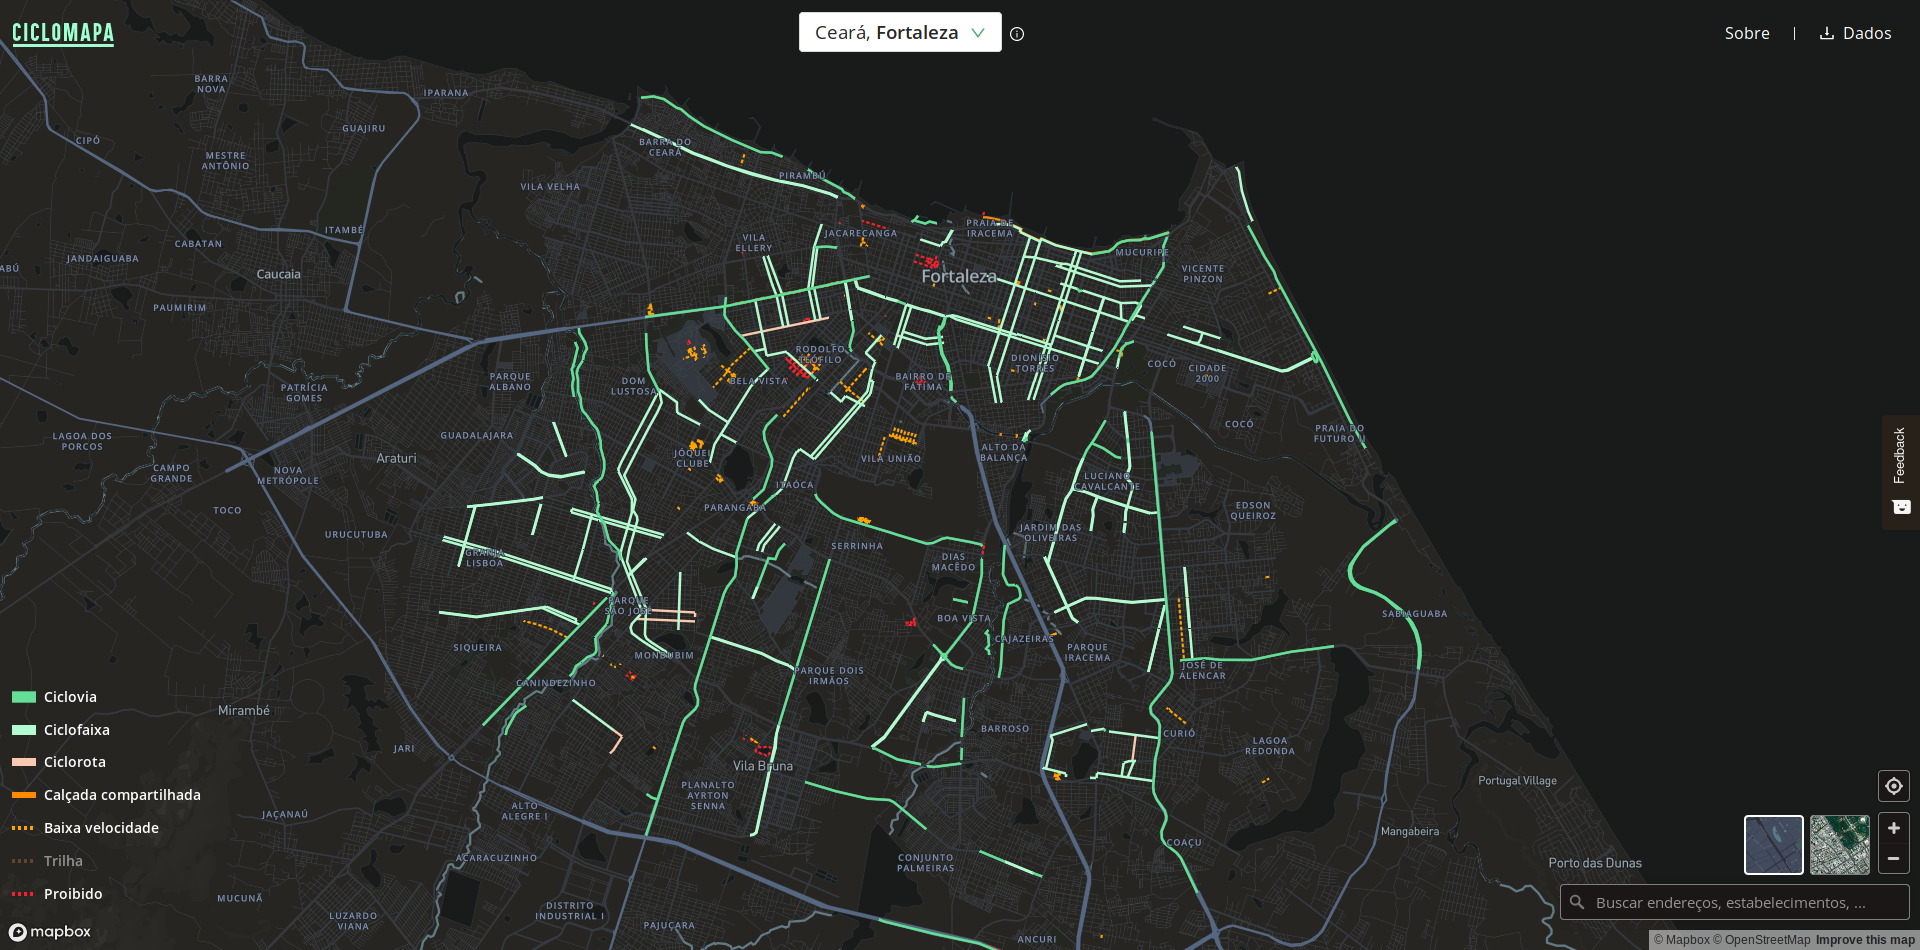
\includegraphics[scale=0.23]{osm_example}
 	\centering
 	\\
 	{Rysunek2. Przykładowy screen z osm}
	\end{figure}
	 
	 Biblioteki: \\
	 
	 
	 
	 
	
	
	
	\newpage
	\renewcommand\refname{Źródła}
	\begin{thebibliography}{}
		\bibitem{vrp} 
		{\hypertarget{vrp}{\textcolor{blue}{
		 Dantzig, George Bernard; Ramser, John Hubert (October 1959). "The Truck Dispatching Problem", https://andresjaquep.files.wordpress.com/2008/10/2627477-clasico-dantzig.pdf}}}
		
		\bibitem{cvrp} 
		{\hypertarget{cvrp}{\textcolor{blue}{T. Ralphs, J. Hartman and M. Galati. "Capacitated Vehicle Routing and Some Related Problems". Some CVRP Slides. Rutgers University. 2001}}}
		
		\bibitem{ag} 
		{\hypertarget{ag}{\textcolor{blue}{
		D. E. Goldberg: Algorytmy genetyczne i ich zastosowania. Warszawa: WNT, 1998. (pol.)}}}
	
		\bibitem{python} 
		{\hypertarget{python}{\textcolor{blue}{
		 Guttag, John V. (12.08.2016). Introduction to Computation and Programming Using Python: With Application to Understanding Data. MIT Press. ISBN 978-0-262-52962-4.}}}
	 
	 	\bibitem{osm} 
	 	{\hypertarget{osm}{\textcolor{blue}{
		https://wiki.openstreetmap.org/wiki/About\_OpenStreetMap}}}
		\bibitem{osm} 
		{\hypertarget{osm_example}{\textcolor{blue}{
		https://wiki.openstreetmap.org/wiki/File:Screenshot\_2019-10-23\_CicloMapa.png
		}}}

	\end{thebibliography}
	
	
	%\end{flushleft}
	
\end{document}